En el siguiente capítulo se presentan las pruebas y los resultados obtenidos a partir de la metodología descrita en el capítulo anterior. Se presentan las pruebas preliminares de comunicaciones para determinar las características óptimas del canal, las pruebas para la estimación de la inclinación que permitieron escoger el método de estimación apropiado y finalmente las pruebas de funcionamiento del prototipo.

\section{Pruebas de comunicaciones}



Una vez escogido el hardware propuesto en la sección \ref{sec:componentes}, se llevaron a cabo una serie de pruebas  para comprobar el funcionamiento de los módulos de comunicaciones y para evaluar las caracacterísticas más adecuadas para el canal de comunicaciones. 

Como se definió en el apartado \ref{sec:protocololora}, el protocolo LoRa implementado en el módulo Ra-02 de Ai-Thinker requiere fijar el valor de los siguientes parámetros:

\begin{itemize}
    \item Factor de propagación.
    \item Ancho de banda.
    \item Potencia.
    \item Tasa de codificación.
\end{itemize}

La prueba consistió en el envío de un paquete de bytes a una distancia de aproximadamente 115 metros, sin línea de vista y con obstáculos de acero y concreto, como se observa en el mapa de la figura \ref{fig:mapalora}.

\begin{figure}[H]
    \centering
    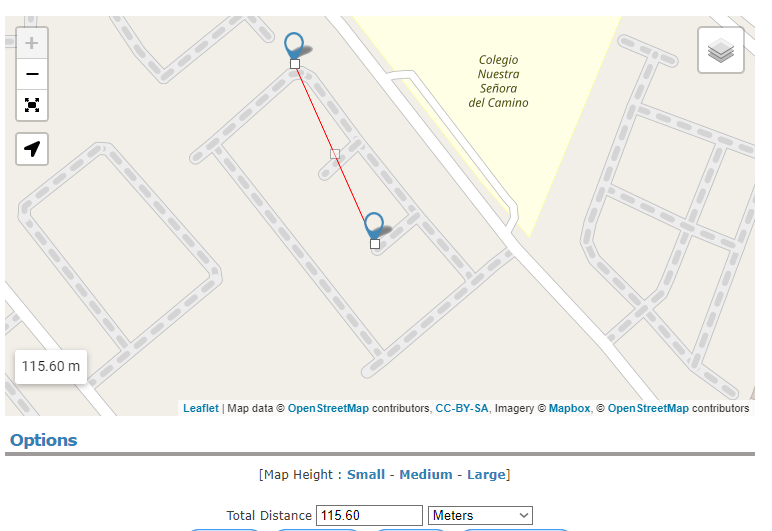
\includegraphics[width = 0.9\textwidth]{imagenes/cap3_resultados/Pruebas LoRa/MapaLora.png}
    \caption{Vista en mapa de distancia máxima de pruebas usando módulo SX1278.}
    \label{fig:mapalora}
\end{figure}

Se modificaron los parámetros del canal y se midió la tasa de paquetes con errores o paquetes corruptos en el receptor. Se realizaron pruebas con los siguientes parámetros fijos:

\begin{itemize}
    \item Frecuencia de operación: 433 MHz.
    \item Tasa de codificación:
    \item Potencia: 10 dBm.
    \item Longitud del preámbulo: 8 bytes.
    \item Tamaño de la carga útil (payload): 128 bytes.
\end{itemize}

Estos parámetros son recomendados por el fabricante del módulo y se mantuvieron constantes durante las pruebas. Estos se confirmaron tras pruebas preliminares en las cuales se observó que para \textit{payloads} mayores a 128 bytes el porcentaje de paquetes cuyo CRC era erróneo (data corrupta) aumentaba considerablemente, siendo 128 bytes un valor que disminuía esta proporción. Los parámetros que se modificaron fueron el factor de propagación, el ancho de banda y el período de envío entre paquetes. Los resultados de las pruebas se presentan en la tabla \ref{tab:resultadoslora}.

% Please add the following required packages to your document preamble:
% \usepackage{graphicx}
\begin{table}[H]
    \centering
    \caption{Resultados de pruebas realizadas con módulo de comunicaciones Ra-02.}
    \label{tab:resultadoslora}
    \resizebox{\textwidth}{!}{%
    \begin{tabular}{|c|c|c|c|c|}
    \hline
    \textbf{Configuración} & \textbf{F. de Propagación} & \textbf{Ancho de banda} & \textbf{Período} & \textbf{Tasa de paquetes perdidos} \\ \hline
    1 & 9 & 125 kHz & 500 ms & 105/500 \\ \hline
    2 & \textbf{7} & 250 kHz & 150 ms & 1/500 \\ \hline
    3 & \textbf{8} & 125 kHz & 150 ms & 300/500 \\ \hline
    4 & \textbf{8} & 250 kHz & 500 ms & 2/500 \\ \hline
    5 & \textbf{8} & 250 kHz & 200 ms & Error de CRC \\ \hline
    6 & \textbf{7} & 250 kHz & 250 ms & 2/500 \\ \hline
    7 & \textbf{7} & 250 kHz & 200 ms & 2/500 \\ \hline
    8 & \textbf{7} & 250 kHz & 150 ms & 2/500 \\ \hline
    9 & \textbf{7} & 250 kHz & 100 ms & Error de CRC \\ \hline
    \end{tabular}%
    }
    \end{table}

Basados en estos resultados, se escogió la configuración 8 para las pruebas de comunicaciones, ya que es la que presenta la menor tasa de paquetes corruptos a la velocidad más alta de envío de paquetes. Esta configuración se utilizó para las pruebas de estimación de inclinación y para las pruebas de funcionamiento del prototipo.

\section{Pruebas para estimación de inclinación}

Para escoger el método de estimación de ángulos, se compararon los siguientes:

\begin{itemize}
    \item Cálculo trigonométrico a partir de mediciones de acelerómetro.
    \item Filtro de Kalman.
    \item Filtro de Madgwick.
\end{itemize}



\section{Pruebas de funcionamiento del prototipo}